\documentclass[11pt]{article}
\usepackage[margin=1in]{geometry}

% Packages we need
\usepackage{amsmath}
\usepackage{mathtools}
\usepackage{amsthm}
\usepackage{float}
\usepackage{graphicx}
\usepackage{listings}
\usepackage{color} %red, green, blue, yellow, cyan, magenta, black, white

% Header packages
\usepackage{fancyhdr}
\fancyhf{}
\pagestyle{fancy}

% Algorithms
\usepackage{algorithmic}
\usepackage{algorithm}

% Formatting document
\setcounter{secnumdepth}{0}
\setlength{\parindent}{0in}
\setlength{\parskip}{0.5em}

% MATLAB code
\definecolor{mygreen}{RGB}{28,172,0} % color values Red, Green, Blue
\definecolor{mylilas}{RGB}{170,55,241}
\lstset{language=Matlab,%
    %basicstyle=\color{red},
    breaklines=true,%
    morekeywords={matlab2tikz},
    keywordstyle=\color{blue},%
    morekeywords=[2]{1}, keywordstyle=[2]{\color{black}},
    identifierstyle=\color{black},%
    stringstyle=\color{mylilas},
    commentstyle=\color{mygreen},%
    showstringspaces=false,%without this there will be a symbol in the places where there is a space
    numbers=left,%
    numberstyle={\tiny \color{black}},% size of the numbers
    numbersep=9pt, % this defines how far the numbers are from the text
    emph=[1]{for,end,break},emphstyle=[1]\color{red}, %some words to emphasise
}

% Commands
\DeclarePairedDelimiter\ceil{\lceil}{\rceil}
\DeclarePairedDelimiter\floor{\lfloor}{\rfloor}
\newcommand{\ws}{\text{ }}
\newcommand{\e}[1]{\times 10^{#1}}

% Header
\lhead{\textsc{CS 5220 -- Aug. 27 Preclass Questions}} % TODO: enter title here
\rhead{\textsc{Eric Gao -- emg222}} % Authors
\setlength{\headheight}{0.5in}
\cfoot{\thepage}

% Title
\title{CS 5220 -- Aug. 27 Preclass Questions} %TODO: enter title here
\author{
  \begin{tabular}{l c l}
    Eric Gao & -- & emg222\\
  \end{tabular}\\
  \rule{\linewidth}{0.4pt}
}
\date{}


\begin{document}
    \thispagestyle{empty}
    \maketitle

    \section*{Question 1}
        Amdahl's law tells us that the speed up is bounded from above by:
        \begin{equation*}
            S(p) \leq \frac{1}{\alpha (1 - \alpha) / p}
        \end{equation*}

        Using this relation, the following plot was produced:
        \begin{figure}[H]
            \centering
            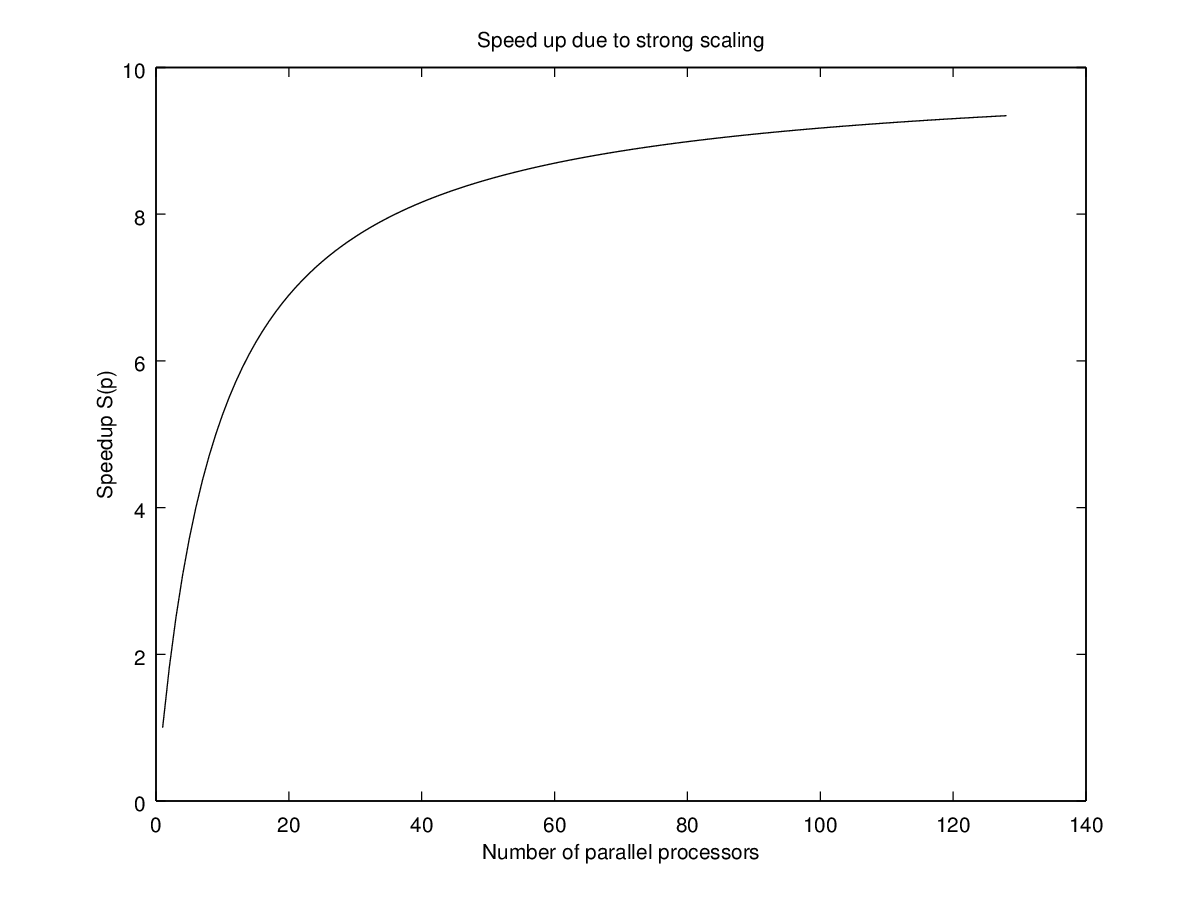
\includegraphics[width=5in]{q1.png}
        \end{figure}

        The code to produce this image was:
        \lstinputlisting[language=Matlab]{q1.m}

    \section*{Question 2}
        You can have up to $p$ workers working at any one time. So the amount to schedule $p$ tasks is: $\alpha p$ time. Therefore, the time to perform $p$ tasks is bounded from above by $\alpha p + \tau$. Therefore, our theoretical maximum throughput is:
        \begin{equation*}
            \frac{p}{\alpha p + \tau}
        \end{equation*}

    \section*{Question 3}
        There are a few circumstances under which it would not be best to tune:
        \begin{enumerate}
            \item When you are not running the code more than once or a few times.
            \item Performance tuning can reduce the readability of code. When it makes code unnecessarily complex, it may not be worth it.
            \item When the code is already running at close to peak performance. Or when you could tune another part of the code that would result an even better speedup.
        \end{enumerate}

    \section*{Question 4}
        We have 60 cores per accelerator and 15 Xeon Phi accelerator boards. Each core on the Xeon Phi board has a clock speed of 1.053 GHz (http://ark.intel.com/products/71992/Intel-Xeon-Phi-Coprocessor-5110P-8GB-1\_053-GHz-60-core). Therefore, assuming we can perform the theoretical maximum of 4 FLOPs per cycle (https://en.wikipedia.org/wiki/FLOPS), we would have the following FLOP rate on just the 15 accelerator boards:
        \begin{equation*}
            15 \text{ accelerators} \times 60 \frac{ \text{cores} }{ \text{acclerator} } \times 1.053\times 10^9 \frac{ \text{cycles} }{ \text{second core} } \times 4 \frac{ \text{FLOPs} }{\text{cycle} } = 3790.8 \text{ GFLOPs}
        \end{equation*}

        We then also have 8 nodes, with 12 cores per node. We also have 2 threads per core due to Intel Hyperthreading. Any core on these 8 nodes has a theoretical maximum clock rate of 3.5 GHz (http://ark.intel.com/products/75283/Intel-Xeon-Processor-E5-2697-v2-30M-Cache-2\_70-GHz). Assuming these specs, the FLOP rate of our 8 compute nodes is given by:
        \begin{equation*}
            8 \text{ nodes} \times 12 \frac{\text{cores}}{\text{node}} \times 2 \frac{\text{threads}}{\text{core}} \times 3.5\times 10^9 \frac{\text{cycles}}{\text{second thread}} \times 4 \frac{\text{FLOPs}}{\text{cycle}} = 2688 \text{ GFLOPs}
        \end{equation*}

        This gives us a total and theoretical maximum FLOP rate of: $3790.8 + 2688 = 6.4788 \text{ TFLOPs}$, or about 6.5 TeraFLOPs per second.

    \section*{Question 5}
        My machine has a Intel Core i7 running clocked at 4.0 GHz. There are 4 cores, with 2 threads per core due to Intel Hyperthreading. Assuming again 4 FLOPs per clock cycle, my machine has a theoretical maximum FLOP rate of:
        \begin{equation*}
            4 \text{ cores} \times 2 \frac{\text{threads}}{\text{core}} \times 4.0\times 10^9 \frac{\text{cycles}}{\text{second thread}} \times 4 \frac{\text{FLOPs}}{\text{cycle}} = 128 \text{ GFLOPs}
        \end{equation*}

\end{document}